\subsection{K-Means}
K-Means is simple and reasonably fast clustering algorithm. K represented the number of cluster the algorithm should create and means refers to the average value of each cluster. Given a set of data their similarity is measured as the value of the Euclidean distance between them. The euclidean distance formula is described for two dimensional data in equation \ref{eq:euclid}, this would be suitable for spatial data in a 2D plane such as an image, whose pixels are located in the dimension x and y. As the K-means algorithm executes, data samples are assigned to the cluster whose average value is closest to its own, the centroids are updated after each round of assignments until their values converge. Initially the average value of all clusters is randomly selected, referred to as cluster centroids. The algorithm to implement the K-means method is outlined in algorithm \ref{algorithm:k_means}.

\begin{equation}
    D(\vec{p},\vec{q}) = \sqrt{(p_1 - q_1)^2 + (p_2 - q_2)^2 +\hdots + (p_n - q_n)^2}
    \label{eq:euclid}
\end{equation} 

\begin{algorithm}
    \SetAlgoLined
    \KwInput{Set of data X of size M} 
    \KwOutput{K sets of clustered data}
    Initialize the desired number of clusters $K$\;
    Intialize a list of $K$ random cluster centroids $\mu$\;
    \While{$\mu$ elements have not converged}{
        \For{i = 0 to M}
        {
            $distOld = \inf$
            \For{$j = 0 to K$}{
                $distnew = euclideanDistance(X[i], \mu_j)$\;
                \If{distNew \le distOld}{
                    $distOld = distNew$\;
                    $\mu_j$.append(X[i])\;
                }
            }
        }
        \For{p = 0 to K}{
            centroidList.append(average($cluster_p$))
        }
    }
    \caption{K-Means Clustering \cite{oreilly_python}}
    \label{algorithm:k_means}
\end{algorithm}

The best result for this method is defined as having the smallest intracluster variance. K-Means is disadvantaged by the implicit trait that it formulates clusters of similar sizes. This happens because the algorithm seeks to minimize variance (spread) in each cluster hence the \q{ideal} centroid placement will form distributions spherically about centroids. This method cannot disentangle overlapping samples that belong in different classes. In Figure \ref{fig:clusters} clear edges between clusters and sphereical distributions can be observed. The algorithm can only implement \emph{hard assignments}, as opposed to a \emph{soft assignment} that consider the probability of a sample's class membership. 



\begin{figure}[H]
    \centering
    \centering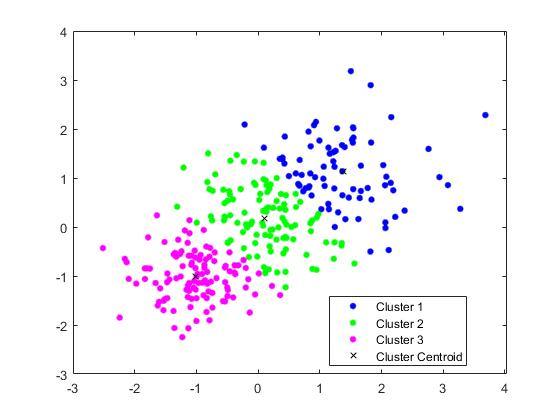
\includegraphics[width=300pt]{kmeans_clusters}
    \caption{K-Means clustering performed on random data.}
    \label{fig:clusters}
\end{figure} 